\documentclass[12pt]{article}

% Package include
\usepackage{url}
\usepackage{graphicx}
\usepackage{fancyhdr}
\usepackage[utf8]{inputenc}
\usepackage[T1]{fontenc}
\usepackage[french]{babel}
\usepackage{color}
\usepackage{lastpage}
\usepackage[export]{adjustbox}
\usepackage{glossaries}
\usepackage[top=1in, bottom=1in, left=1in, right=1in]{geometry}
\usepackage[hidelinks]{hyperref}
\usepackage[nodayofweek,level]{datetime}
\usepackage[backend=biber, style=numeric, sorting=none]{biblatex}
\usepackage[toc,page]{appendix}
\usepackage[labelsep=colon]{caption}
\usepackage{csquotes}
\usepackage{pdfpages}
\usepackage{listings, listings-rust}
\usepackage{lstautogobble}

%------------------------------------------------------------------------------%

% Hyper-link setup
\hypersetup{
	colorlinks = false, %Colours links instead of ugly boxes
	urlcolor   = blue,  %Colour for external hyperlinks
	linkcolor  = blue,  %Colour of internal links
	citecolor  = red    %Colour of citations
}

%------------------------------------------------------------------------------%

% General definitions

% Repositories
\def\sources    {src}
\def\images     {resources/images}
\def\glossaries {resources/glossaries}
\def\biblio     {resources/bibliography}

% Project propreties
\def\genre      {Rapport de Stage de Fin d'Etudes}
\def\subject    {Mise en place d'un service de communication au standard MQTT hébergé au sein d'un environnement kubernetes}
\def\audience   {Génie Logiciel}

% TO-DO shortcut
\def\TODO   {
                \begin{center}
    				\Huge{\bfseries Fill in ...}
    			\end{center}
    		}

% Project Data
\def\creator        {Ihsen Charfi}
\def\establishment  {INSAT}
\def\company        {Mobile Devices Ingénierie}
\def\mentor         {Jeremy HEATER}
\def\correspondent  {Riadh ROBENNA}

% Set project variables

\title{\genre{}}
\author{\creatpr{}}
\date{\today}

%------------------------------------------------------------------------------%

% General page configuration

% Style fancy
\pagestyle{fancy}

% Undef header and footer
\fancyhf{}

% Special definiton for footer
\lfoot{\textsc{\company}}
\cfoot{\textsc{\audience}}
\rfoot{\thepage}

% Set header and footer rules
\renewcommand{\headrulewidth}{0pt}
\renewcommand{\footrulewidth}{1pt}

% Fix non-break space definiton
\DeclareUnicodeCharacter{00A0}{ }

% Set figure caption display
\makeatletter
\renewcommand{\fnum@figure}{Fig.\thefigure}
\makeatother

%------------------------------------------------------------------------------%

% Glossary definition

% Make glossary entries clickable links
\glsenablehyper

% Import glossaries from file
\newglossaryentry{mdi} {
	name=MDI,
	description={Mobile Devices Ingénierie}
}
\newglossaryentry{md30} {
	name=MD30,
	description={Mobile Devices 30 : le nom du nouveau protocol de communication }
}
\newglossaryentry{INSAT} {
	name=INSAT,
	description={Institut National des Sciences Aplliquées et de la Technologie}
}
\newglossaryentry{CC} {
	name=CC,
	description={CloudConnect}
}
\newglossaryentry{CN} {
	name=CN,
	description={CloudNext}
}

\newglossaryentry{poc} {
	name=PoC,
	description={Proof of Concept}
}
\newglossaryentry{mdi21} {
	name=MD21,
	description={Mobile Device 21 : le protocole de communication actuel de MDI}
}
\newglossaryentry{obd} {
	name=OBD,
	description={ON Board Diagnostics}
}
\newglossaryentry{BS} {
	name=BS,
	description={Binary Server: service de communication entre Cloud et boîtiers}
}
\newglossaryentry{gdpr} {
	name=GDPR,
	description={General Data Protection Regulation - Réglement Général sur la protection des données\cite{gdpr} }
}
\newglossaryentry{asn1} {
	name=ASN.1,
	description={Abstract Syntax Notation One: Syntxe de grammaire utilisé pour décrire les protocoles de communication.}
}

% Create glossaries
\makeglossaries

%------------------------------------------------------------------------------%

% Bibliography definition

\bibliography{\biblio}

%------------------------------------------------------------------------------%

% The document

\begin{document}

	% Disable anchors for title page (Numbering duplication issues)
	\hypersetup{pageanchor=false}

	\begin{titlepage}
    \newgeometry{top=4cm, bottom=3cm, left=1in, right=1in}
    \begin{center}
        \Large \textsc{\establishment}\\[1cm]
        \Large \textsc{\company}\\[1cm]
        \begin{center}
            \raisebox{-0.2\height}{
\includegraphics[width=0.2\textwidth]{\images/mdi_logo.jpeg}}
        \end{center}
        \hspace{0.15\textwidth}
    \end{center}
    \begin{center}
        \Large{Rapport de stage d'ingénieur}\\[0.5cm]
        \line(1,0){410}\\
        \huge{\bfseries \subject}\\
        \line(2,0){390}\\[2cm]
        \color{red}\Huge{\textsc{\audience}}\\[2cm]
    \end{center}
\begin{flushleft}
    \begin{itemize}
        \renewcommand{\labelitemi}{$\bullet$}
        \item \creator
        \item Diplôme préparé : Ingénieur en Génie Logiciel
        \item Encadrant de stage en entreprise: \mentor
        \item Responsable de stage à l'INSAT : \correspondent
        \item Durée du stage : Du \formatdate{13}{03}{2018} au \formatdate{31}{8}{2018}
        \item Date de remise du rapport : Le \today{}
    \end{itemize}
\end{flushleft}
\restoregeometry
\end{titlepage}


	% Reactivate anchors for title page (Numbering duplication issues)
	\hypersetup{pageanchor=true}

	% Use roman numerals for front matter
	\pagenumbering{Roman}

	\addcontentsline{toc}{section}{Remerciements}

\thispagestyle{plain}

\begin{center}
    \huge \textsc{Remerciements}\\[2cm]
    \large
        J'aimerai, au debut de ce rapport, remercier tous ceux qui ont contribué
        à rendre ce stage une expérience riche et épanouissante, en particulier,
        mon encadrant coté entreprise \mentor{} et mon encadrant coté INSAT \correspondent.\\[1cm]


        Je tiens aussi à remercier toutes les personnes qui m'acompagnaient au cous du parcours à l'INSAT, mes binomes
        mes amis les plus proches qui se reconnaissent et toute personne qui m'a soutenu.\\[1cm]


        Enfin, je remercie....\\[1cm]
\end{center}


	% Create table of contents
	\addcontentsline{toc}{section}{Sommaire}
	\tableofcontents

	\pagebreak

	% Use arabic numerals for main matter
	\pagenumbering{arabic}

	\section{Introduction Générale}
    Paragraphe sur la télématique des voitures , la voiture connectée, 
    la tendance des clouds et systèmes big data ...


    La télématique est née de la convergence des progrès de l'informatique embarquée et 
    des télécommunications. Dans le domaine des transports, elle désigne les dispositifs 
    permettant la production, l'émission, la réception, le traitement et la représentation 
    des données de manière automatisées.


	\section{Présentation du contexte du projet}
    \subsection{\company{}}
        \subsubsection{Qui est \texorpdfstring{\gls{mdi}}{MDI}?}
            \company{}\cite{mdi_site}, un des leaders mondiaux de la télématique, est une entreprise
            française spécialisée dans les systèmes embarqués pour l'automobile.
            L’entreprise dont le siège est situé en région parisienne (à Villejuif) a depuis à peu près
            15 ans, conçu et développé des boîtiers connectés aux véhicules par port OBD (On
            Board Diagnostics).\\[0.3cm]
            Actuellement, \gls{mdi} comprend une cinquantaine d’employés répartis dans plusieurs
            pays dont la France, les États-Unis et l’Afrique du sud. Avec un chiffre d’affaire de
            plusieurs dizaines de millions d’euros et plus d’un million de boîtiers déployés dans le
            monde.\\[0.3cm]


            ((((((((((((((((((((((((((((((figure : carte du monde montrant les pays où se trouvent MdI ( fr , USA , AS ) et les 
            pays ou les OBD sont déployés ( les clients:  (Autriche, Belgique, Bulgarie, Croatie, Chypres, République Tchèque, Danemark, Estonie, ETats unies, Finlande, France, Allemagne, Grèce, Hongrie, Ireland, Italie, Lettonie, Lituanie, Luxembourg, Malte, Pays bas, Pologne, Portugal, Romanie, Slovaquie, Slovénie, Espagne, Suède, Suisse, Grande Bretagne))))))))))))))))))))))))))))))))
            \begin{figure}[ht]
                \centering
                
\includegraphics[scale=1]{\images/cartemonde1.jpg}
                \caption{Les pays où circulent des véhicules ayant des OBD déployés }
            \end{figure}


            
            Les clients de Mobile Devices Ingénierie sont ainsi réparties partout dans l'Europe et les Etats Unies. 
            En effet, ils occupent différents secteurs d’activités tels que :\\
            \begin{itemize}
                \renewcommand{\labelitemi}{$\bullet$}
                \item Des applications embarquées de gestion de flottes de taxis 
                \item Des compagnies d’assurances 
                \item Des compagnies de navigation et d'info trafic 
                \item Des revendeurs qui adaptent les produits MDI à leurs services et qui disposent d’un accès à certains marchés de par leur histoire ou leur image de marque.
            \end{itemize}


        \subsubsection{Domaine d'activité et Stratégie }
            L’objectif de l'entreprise est de devenir le leader mondial pour l'acquisition, le
            traitement, l'enrichissement et l’échange des données techniques de véhicules
            connectés.\\[0.3cm]

            Mobile Devices Ingénierie a pour secteur d’activité la télématique embarquée pour l'automobile. 
            Concrètement, cela consiste à proposer des solutions techniques permettant l'échange d'informations 
            entre un ou plusieurs systèmes de gestion centralisés et une flotte de véhicule qui y est rattachée 
            et connectée en temps réel.
            Ces informations sont ensuite récupérées en temps réel et peuvent être envoyées 
            vers les serveurs de l’entreprise ou des clients. \\[0.3cm]

            \begin{figure}[ht]
                \centering
                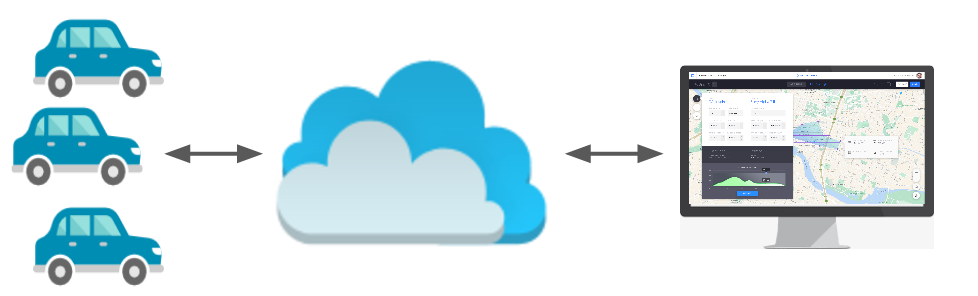
\includegraphics[scale=0.4]{\images/carcloud.png}
                \caption{Schema représentant le circuit des données remontés  }
            \end{figure}
            
            L’activité principale de Mobile Devices Ingénierie se résume à la mise en place de solutions techniques 
            afin d’effectuer le suivi de véhicules et la gestion de flottes. Les produits de l'entreprise permettent 
            de récupérer des données telles que la vitesse, la consommation, le type de conduite et même de prévenir 
            des accidents.
            Ces mêmes données permettent ensuite, par exemple pour certaines entreprises, d’étudier la conduite 
            des véhicules et leurs différents paramètres comme suivre un déplacement et/ou quantifier la consommation 
            dans le cas d’une gestion de flotte. \\
            Ces données peuvent aussi servir à étudier le type de conduite dans le cas d’une compagnie d’assurance. 
            La société compte aussi d'autres activités comme la commercialisation des boîtiers pouvant offrir l’aide 
            à la navigation servant par exemple aux Taxis.
            Les entreprises clientes peuvent aussi reprogrammer une partie de leurs boîtiers afin de récupérer des données 
            spécifiques et les transférer vers des serveurs distants. \\[0.3cm]

            Par la nature même de l’activité, l’entreprise apporte à ses clients des solutions
            innovantes permettant de concilier le développement économique et la préservation de l’environnement.
            En effet, ses solutions permettent de mettre en œuvre le contrôle
            de baisse de la consommation énergétique, de l’empreinte carbone des
            véhicules et du risque environnemental associé.\\[0.3cm]
            Dans le cadre de son développement durable, la protection de l’environnement est une
            préoccupation fondamentale pour \gls{mdi}. L’éthique, l’équité et la diversité sont des
            facteurs de progrès qui contribuent à améliorer les résultats économiques ainsi que le
            climat social, éléments clefs d’un développement durable pour \company{}.

        \subsubsection{Organisation et produits}
        L’entreprise suit un schéma d’organisation hiérarchique fonctionnelle composée d’une division classique du 
        travail par fonctions. Elle est constituée d’un dirigeant et ensuite d’une équipe de collaborateurs ayant 
        différentes fonctions : commerciale, comptable, financière, ressource humaine, production, etc. 
           Quant au côté technique, \gls{mdi} articule plusieurs types d'équipes: \\
            \begin{itemize}
                \renewcommand{\labelitemi}{$\bullet$}
                \item L’équipe \textbf{Production} en charge de la production et la livraison des produits
                \item L’équipe \textbf{Core} en charge de « Morpheus » (le système d’exploitation applicatif du boîtier)
                \item L’équipe \textbf{Système} en charge du système d'exploitation linux
                \item L’équipe \textbf{Pre-Sales} en charge du support clients et accompagement des commerciaux
                \item L’équipe \textbf{Serveur} en charge du cloud, au sein de laquelle j'ai effectué mon stage
            \end{itemize} 
            
            \vspace{0.5cm}

        Ces équipes travaillent sur différents projets autour des produits hardwares et softwares: 
            \begin{table}[h!]
                \centering
                \begin{tabular}{|p{5cm}|p{5cm}|}
                    \hline   Les produits Hardwares & Les produits Softwares \\
                    \hline
                    \begin{itemize}
                        \renewcommand{\labelitemi}{$\bullet$}
                        \item munic.io
                        \item municMax
                        \item \gls{obd} Dongle
                    \end{itemize} 
                   & 
                    \begin{itemize}
                        \renewcommand{\labelitemi}{$\bullet$}
                        \item Morpheus OS
                        \item CloudConnect
                        \item CloudNext
                    \end{itemize}\\
                    \hline 
                \end{tabular}
                \caption{Tableau des produits MDI}
                \label{table:1}
            \end{table} \\

            \vspace{0.3cm}

            Les produits Hardwares sont intégrés dans les véhicules et récolte des informations sur 
            la vitesse, la position, le niveau de carburant, la pression des pneus, etc..  à un instant t donnée.
            En général nous appelons ces produits hardwares “les boîtiers” qui doivent être intégrés dans 
            les véhicules et déployés  dans le système cloud. \\ [0.1cm]
            Quant aux produits Softwares, il y a le Morpheus OS qui présente le système d'exploitations des boitiers. 
            D'autre part,les clouds CloudConnect et CloudNExt qui offrent un ensemble de services aux clients 
            et qui sont développés et maintenus par l'équipe Serveur. On détaillera plus sur ces deux produits dans le prochain chapitre. 
       
        \subsection{Présentation du projet}
        \subsubsection{Contexte du projet}
            Mon sujet principal de stage est la conception et développement du nouveau composant du Cloud. Ce composant représente 
            le point d'entrée des données au cloud. Il assure la communication entre le cloud et les boitiers. 
            Le composat actuel porte le nom de \gls{BS} - acronyme de Binary Server. Il est intégré seulement dans CloudConnect.
            \begin{figure}[ht]
                \centering
                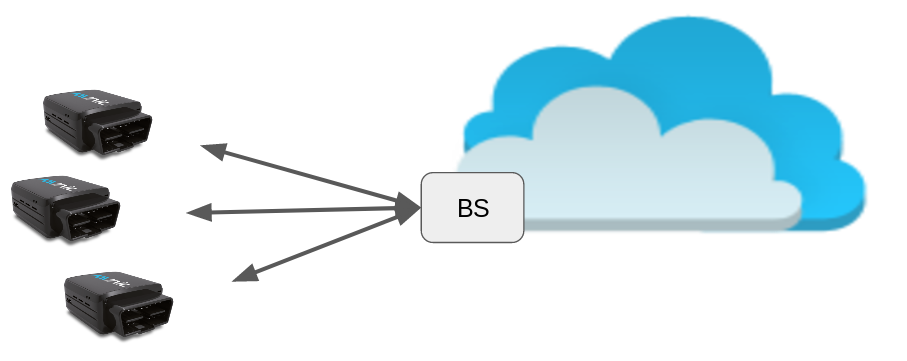
\includegraphics[scale=0.2]{\images/bs.png}
                \caption{BS le seul point d'entrée des clouds }
            \end{figure}
           
        \subsubsection{Problématique}
            Plusieurs facteurs  rendent le développement d'un noouevau composant cloud une necessité. 
            \\Dans l’architecture actuelle, les deux cloud sont totalement indépendants mais ils reçoivent les données 
            de la même source \gls{BS} malgrès la différence entre les deux formats de messages. \\ 

            D'autre part , pour une raison commercial, le nouveau protocol migre d'un protocol fait maison vers un protocol standardisé. \\
            Un standard permet de bénéficier des librairies existantes sur le marché et donc de gagner en temps d'intégration puisque 
            il' n y aura pas le besoin de faire du développement à zéro.
            MQTT n'étant pas propriétaire, les partenaires ou clients savent également comment celui-ci est conçu. Ce qui n'est pas le cas 
            pour \gls{mdi21} \- le protocole actuel fait maison \-  donc cela permet de rassurer le client. 
            Le "standard MQTT" permets également de laisser d'autres boitiers se connecter à notre plate-forme plus facilement 
            plutot que d'implémenter notre protocole propriétaire dont ils n'ont meme pas les sources. \\
            Donc la possibilité de gagner la confiance de plus de clients et de s'ouvrir à des marchés potentiels.


         \subsubsection{Objectifs}
           Suite à cette problématique \gls{mdi} a mis en place le projet \gls{md30} pour mettre en place la solution.
           Les objectifs du projet consiste à : 
            \begin{itemize}
                \renewcommand{\labelitemi}{$\bullet$}
                \item concevoir et réaliser un nouveau protcole de communication entre boitier et cloud
                \item mettre en place un nouveau composant \gls{BS}
                \item faire une étude de faisabilité et de performance de l'intégutilisation du protocol MQTT 
                comme protocol de communication.
                \item Le support du format de données CloudNext par le nouveau BS
            \end{itemize} 

    \subsection{Méthodologies de travail}
        \subsubsection{Cycle itératif }
            Le mode itératif est une méthodologie de développement différente des méthodes classiques( modèle en cascade, modèle en V ).
            Elle tente de formaliser une méthode plus pragmatique et maniable que ces derniers. 
            \begin{figure}[ht]
                \centering
                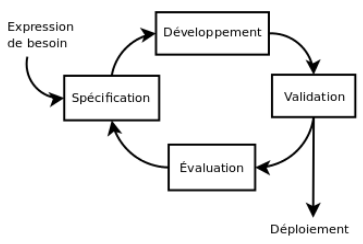
\includegraphics[scale=0.8]{\images/cycleiteratif.png}
                \caption{Le processus du cycle itératif}
            \end{figure}
           
            \vspace{0.2cm}

            Cette méthode présente 6 étapes marquante : 
            \begin{itemize}
                \renewcommand{\labelitemi}{$\bullet$}
                \item L’expression de besoin: où les exigences sont mis en place. L’idée reste que 
                les informations en entrée peuvent être modifiées par la suite du processus itératif.\\
                Le cercle du processus itératif: 
                \begin{itemize}
                    \renewcommand{\labelitemi}{$\bullet$}
                    \item  La spécification technique du besoin 
                    \item  Le développement : la période où on implémente la spec
                    \item  La validation : une étape qui est marqué par les tests.C’est l’ensemble des tests qui 
                    permettent de s’assurer que le développement effectué correspond bien à ce qui était attendu.
                    \item  L’évaluation : Cette étape sert à effectuer un retour sur les fonctionnalités laissés. 
                    Ceci sert comme des informations d’entrée pour un nouveau cycle.
                \end{itemize} 
                \item Déploiement : l’étape finale qui consiste à ce que les livrables validés sont livrés.  
            \end{itemize}

             \vspace{0.5cm}
            
            Ce type de cycle de développement est le plus souple des méthodologies:
             chaque itération permet de s’adapter à ce qui a été appris dans les itérations précédentes et 
             le projet fini peut varier du besoin qui a été exprimé à l’origine.\cite{cycle_iteratif} \\
            
            Vu la nature du projet qui part plutôt vers une étude de faisabilité avec des critères de performances, 
            l’expression des besoins peuvent être redéfinies pendant ce temps. Il est préférable de suivre une méthodologie 
            souple d’où le choix de telle méthodologie. 
            


        \subsubsection{MD30 un travail d'équipe}

        le projet MD30 présente le nouveau protocole de communication entre les boîtiers OBD et le CLoud et donc le projet 
        invoque les boîtiers ainsi que le point d entrée du cloud. \\ [0.3cm]
        Le projet MD30 engage 5 personnes dans deux différentes parties : 
        \begin{itemize}
            \renewcommand{\labelitemi}{$\bullet$}
            \item 2 personnes sur MD30 côté Serveur
            \item 3personnes sur MD30 côté Core
        \end{itemize} 
         
        \vspace{0.2cm}
        
        Même si le coeur de développement des deux parties est totalement indépendant l’un de l'autre. Les deux parties doivent 
        rester synchroniser sur l'avancement de chaque partie afin d'avancer dans le projet en phase.  
        

	\section{Etat de l 'art}
   Cette partie concerne plus l architecture global des clouds. Leurs évolutions 
   au cours du temps ce qui mettra le point sur le besoin de la création d un nouveau 
   point d entrée.   

    \subsection{Le premier Cloud de MDI}
        \gls{CC} est le premier cloud fait maison de \gls{mdi} qui englobe un ensemble 
        de services pour les clients... L'architecture globale de ce cloud est comme le montre 
        le shema suivant: 

        \begin{figure}[ht]
            \centering
            \includegraphics[scale=0.8]{\images/mos_overview.png}
            \caption{Aper\c cu MOS}
        \end{figure}

        \gls{CC} comporte plusieurs composants : 
        \begin{itemize}
            \renewcommand{\labelitemi}{$\bullet$}
            \item  un \gls{BS} qui est le composant d'échange de messages entre le cloud et 
            les OBD. Il consiste le point d'entrée du cloud.
            \item  un broker de message pour les systèmes Big Data
            \item  un ensemble de services qui sont accéder à partir de APIV3 
            \item une base de données pour le stockage des données 
            \item un dashboard pour l affichage des données et l acces visuel 
            des services au clients 
        \end{itemize}
       
    \break

    \subsection{De \gls{CC} à \gls{CN}}
        Exprimer le besoin du changement d'architecture. 


       

        \vspace{0.2cm}

       

    \subsection{Communication entre composants}
       mos  présente deux méthodes principales de communication entre les
        composants:
        \begin{itemize}
            \renewcommand{\labelitemi}{$\bullet$}
            \item Communication par évènements: Un composant produit un Event,
                et tous les listeners le re\c coivent. Cela est fait par l'intermédiaire
                d'un broker.
            \item Appels API: Chaque composant expose une API pour les composants
                avec authorisation. Le composant a plusieurs choix de méthodes de
                communication (MsgPck, TCP Socket).
        \end{itemize}

        \vspace{0.2cm}

        \begin{figure}[ht]
            \centering
            \includegraphics[scale=0.8]{\images/broker_pattern.png}
            \caption{Le broker MOS}
        \end{figure}

        \subsection{format de données du cloud }

        Track : 
        Message : 
        

        message track 

        Paragraphe sur le language Go : 
        Go\cite{rust_site} est un jeune language de programmation système
        fascinant. Ce language compilé hérite des idées des paradigmes de
        programmation impérative et fonctionnelle. Il définit des concepts et
        des règles qui assurent à l'utilisateur des binaires "safe".\\[0.3cm]
        Rust ne sacrifie pas la performance contre la sûreté. Il a des
        performances similaires à celles de C et C++. En fait, ses plus grands
        partisans espèrent qu'il va détrôner C!
      


	\section{itération 1 : nouveau BS au standard MQTT}
        \gls{mdi}, étant une entreprise innovante en télématique, doit toujours
        suivre et avancer les nouvelles technologies. Une de ces technologies
        est le protocol de communication standard des objets connectés: le MQTT.

        ...
        


    \subsection{Descriptif du protocole:Le standard MQTT, l'essentiel à savoir}
    D’apres la specification officielle MQTT \cite{mqtt_site},
    le standard MQTT est un protocole de transport de message Client/serveur sous le pattern de Publication/Souscription 
    “ Publish/ Subscribe”. 
    C'est un protocole léger , ouvert, simple et désigné d’être facile à implémenter. \\
    Ces caractéristiques le rend idéal à être utilisé dans plusieurs situations, surtout pour la communication Machine 
    to MAchine M2M et pour l’internet des objets IoT. Des contextes où la faible empreinte du code est requise ainsi 
    qu’une bonne bande passante.     \\
    
       
    \textbf{Qu’offre MQTT ? }\\

    \begin{itemize}
        \renewcommand{\labelitemi}{$\bullet$}
        \item L’utilisation du pattern de message “ Publication/Souscription” qui offre 
        des distributions un-à-plusieurs ( one-to-many) et le découplage de ces deux parties.    
        \item 3 Qualités de service QoS pour la distribution des messages . 
        \item Un échange de protocol minimisé pour réduire le trafic  du réseau      
        \item Un mécanisme pour notifier les parties intéressées lors d'une déconnexion anormal    
    \end{itemize}   
    \bigskip 
    En cas de besoin de plus de détails sur le standard, consultez la partie Annexes. Elle comporte des eclaicissements 
    sur le standard MQTT.\\

    \textbf{En quoi MQTT sera meilleur ?  } \\
    Pour répondre à une telle question il faut comparer entre MQTT et le protocole de \gls{mdi21} comme le montre le tableau \ref{table:mqttvsmd21}
    de la page \pageref{table:mqttvsmd21}.
    \begin{table}[h!]
        \centering
        \begin{tabular}{|p{5cm}|p{5cm}|p{5cm}|}
            \hline
            \centering

               & MQTT & \gls{mdi21} \\
            \hline
            Logique & standardisée & fait maison  \\
            \hline
           Protocole basé sur & TCP/IP & TCP - UDP\\
            \hline 
            Couplage entre BS et consommateurs & Broker découplé des consommateurs & couplage fort \\
            \hline
        \end{tabular}   
        \caption{Tableau de comparaison : MQTT vs MD21}
        \label{table:mqttvsmd21}
    \end{table} \\
       
    \break

    \subsection{Specifications techniques \& Implémentation}
       
        Le Point d’entrée du cloud ou BS se charge de deux principales fonctionnalités. 
        \begin{itemize}
            \renewcommand{\labelitemi}{$\bullet$}
            \item  \textbf{Transfert de données :} où ils gèrent les connexions avec les boîtiers.
            \item  \textbf{Traitement de données :} encodage/décodage des données de messages selon le format de données du cloud.
        \end{itemize}

        Puisque le standard repose sur le découplage entre le publisher et subscriber, la conception doit prendre 
        en compte  un broker MQTT pour assurer cette notion. 
        La conception est présenté par la figure suivante .. 

 ********* Insertion d une figure de la conception ************** \\
        Le BS aura deux parties importantes qui sont le transfert des données et l'encodage pour le broker.

    \subsubsection{Recherche \& état de l'art}
            

        Il existe quelque large implémentation de MQTT comme Facebook Messenger par example, mais aussi de nombreux 
        outils monétisés et d'autres open source.
        Il y a aussi un projet Eclipse active, "Paho", qui offre une implémentation scalable , open source pour 
        différents langage de programmation comme Java , 
        C, C++ , Python , JavaScript , C\# et Go lang. \\
        Il existe plusieurs implémentations qui sont réunis dans cette référance \cite{mqtt_choix} publié par un des membbre de la communauté de MQTT et qui les comparent selon plusieurs critères. 
        Pour effectuer un bon choix satisfaisant de toute ce    s propositions, il faut bien demander les critères de l'entreprise en premier lieu 
        sur lesquels on se base. \\
        
        {\centering
        \textbf{A la recherche d'un broker MQTT! } \\}
        \vspace{0.2cm}
        Comme la stratégie de l entreprise est de réduire les coûts, nous éliminons les choix d'outils payants. \\
        D'autre part, le support de QoS 2 n'est pas exigé vue que l'échange de message en QoS 2 est trés couteux. 
        Tandis que le QoS 1 est indispensable pour profiter du système des ack.\\
        Un autre critère est la charge des connexions du broker. L'un des objectifs de \gls{md30} est d'augmenter le support 
        en charge du nouveau BS ce qui revient dans ce cas à étudier la charge du broker MQTT en question. 
        Ceci peut être effectué de deux manières : 
        \begin{itemize}
            \item Augmenter le support en charge du Broker par rapport au \gls{BS} de \gls{mdi21}, sachant que
            le support du BS actuel est de ... 
            \item Assurer la scalabilité du broker ce qui revient à choisir dés le début un broker scalable.
        \end{itemize} 
        \vspace{0.3cm}
        En se basant sur ces critères, nous éliminons déjà beaucoup de choix pour rester avec les implémentations des projets 
        open source qui ont implémenté la QoS 1 ainsi qu'une solution pour la sclalabilité du broker. En plus il faut que le projet soit mis 
        à jour avec une communauté qui le supporte.  
        Nous nous retrouvons alors avec 2 choix qui répondent à nos critères : 
        \begin{itemize}
            \item HmQ : Broker MQTT open source développé en Go lang. 
            \item Mosca : Broker MQTT open source déeloppé en Node.JS. 
        \end{itemize} 
        
        Afin de déterminer lequel de ces brokers sera choisi il faut bien vérifier qu il répondent aux attentes en effectuons quelques tests. 
        Pour ce faire nous avons intégrés les brokers dans la chaine de transfert des données jusqu' à lentrée dans le cloud - 
        c'est à dire le push dans kafka.


        \subsubsection{Développement effectué}
            il faut tester les différents particularités du standard MQTT. 
            \begin{itemize}
                \item le wildcard : 
                \item le support de lastwill : 
                \item le support de QoS 1 
                \item le support 
            \end{itemize} 
           
            Tous ceci ont été vérifié en résumant dans le tableau suivant : 

    \subsection{Tests \& Performance}
    \subsubsection{Virtualisation avec Docker}
    À l’aide de conteneurs, tout ce qui est nécessaire pour faire exécuter un logiciel est emballé
    dans des conteneurs isolés. Contrairement aux machines virtuelles, les conteneurs ne regroupent
    pas un système d’exploitation complet : seules les bibliothèques et les paramètres requis pour
    que le logiciel fonctionne sont nécessaires.\\
    Cela permet d’avoir des systèmes autonomes, légers et garantit que les logiciels fonctionne-
    ront toujours de la même manière, quel que soit l’endroit où ils sont déployés.

    \textbf{Docker}
    Docker est une technologie, un "runtime" pour les conteneurs. Il est aussi une plate-forme
    pour le développement, l’expédition et l’exécution d’applications. Il permet de séparer
    les applications de l’infrastructure afin de livrer rapidement un logiciel. \\

    Avec Docker, on gère l’infrastructure de la même façon qu’on gère les applications.
    En profitant des méthodologies de Docker pour l’expédition, le test et le déploiement rapide
    du code, on peut réduire considérablement le délai entre l’écriture du code et l’exécuter en
    production.\\
    \textbf{Comment docker construit ces conteneurs isolés ?} \\
    \begin{itemize}
        \item \textbf{Isolation du système de fichiers} : chaque conteneur s’exécute dans un système de fichiers
        racine complètement distinct.
        \item \textbf{Isolation des ressources} : les ressources système comme CPU et mémoire peuvent être
        attribuées différemment à chaque conteneur.  Ceci présente la principale motivation pour tester les performances de chaque composant.
        \item \textbf{Isolation de réseau}  : chaque conteneur de processus s’exécute dans son propre espace de
        noms de réseau, avec une interface virtuelle et une adresse IP propre.
    \end{itemize}

    la figure .. montre l’optimisation en ressources qu’offre la virtualisation avec la technologie
    des conteneurs par rapport à la technologie de machine virtuelle et hyperviseur.

    \begin{figure}[ht]
        \centering
        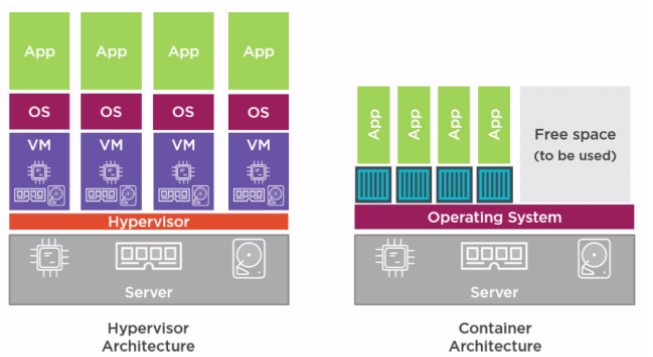
\includegraphics[scale=0.6]{\images/dockervsvirt.png}
        \caption{L'optimisation de docker par rapport à la machine }
    \end{figure}

    \subsubsection{Evaluation}

    Après avoir fini le développement et les tests de la première itération. 
    On évalue le système par rapport à nos exigences globaux du système. 
    Néanmoins lors de cette évaluation on est face à plusieurs problématiques qu il faut pas négliger. 

    \begin{itemize}
        \renewcommand{\labelitemi}{$\bullet$}
        \item Le coût de communication sera élevé, car ça sera des paquets tcp dans des paquets MQTT 
        \item L'ajout du maintien d’un nouveau broker avec sa BD: ceci ajoute de la complexité à gérer.
        \item La manière de consommer depuis le broker: 
    \end{itemize}

    Différentes manières pour effectuer la consommation : 

    Pour chaque manière on étudie les avantages et les inconvénients ... 



    \textbf{Synthèse :}
    Cette première itération nous a prouvé la limite de MQTT pour le projet MD30. Elle sert comme une étude 
    sur la faisabilité d'intégration du standard dans le projet.
    La question qui se pose est , quelles sont les fonctionnalités MQTT que MD30 exige par rapport aux 
    diverses fonctionnalités offertes par MQTT ? = > ils sont peu : 
    Ce que MD30 exige de tout cela n’est que le mécanisme des acks qui sont traités par les headers des messages MQTT. 
    Donc ajouter des bytes de plus comme étant un header dans le nouveau format de message du boîtier permet ce mécanisme. 
    => une implémentation fait-maison de ça fera l'affaire. \\




    \textbf{Conclusion} \break
            Après avoir fait une évaluation de la première itération et faire l étude de coût et performances de MQTT, 
        nous nous rendons compte que ce dernier est tellement riche en exigences divergente des exigences de MD30 et 
        donc l'adopter tel qu il comme le protocole de communication de MDI n’était pas la bonne solution. 


    



  



	\section{Itération2: nouveau BS englobant TCP serveur}
    \subsection{Spec}
    
    Cette partie repose sur la modification des exigences et la nouvelle Conception
        \subsubsection{L'évolution des exigences}
       
            Après avoir fait l’évaluation des résultats de performance 
            de la 1ere itération du projet, on a redéfinit les spécifications du projet. 
            Le tableau suivant montre la différence des exigences entre les deux itérations:
            \\
            \begin{table}[h!]
            \centering
            \begin{tabular}{|p{3cm}|p{3cm}|p{4cm}|p{5cm}|}
                \hline
                \multicolumn{4}{|c|}{Les changements des exigences } \\
                \hline   & Itération1 & Itération2 & Avantage de cette évolution\\
                \hline
                Protocol de communication & MQTT & TCP avec le support de MQTT &
                Moins coûteux par rapport aux paquets échangés, tout en gardant 
                la possibilité de connecter le boîtier à un serveur MQTT \\
                \hline
                Architecture du BS  &  Un cluster de brokers MQTT avec des 
                subscribers des tracks et publishers d’events.  & Un cluster de 
                TCP serveur qui gèrent les connexions, traitent les message échangés 
                et envoient/re\c coivent les msg à/de kafka. & Moins coûteux par 
                rapport aux instances à gérer. 
                Plus facile à gérer un seul composant au BS. 
                Pas de complexité à dispatcher les subscribers quand on monte de charge.\\
                \hline 
            \end{tabular}
            \caption{Tableau de comparaison des exigences du projet}
            \label{table:3}
        \end{table} \\
        La spécification téchnique peut être divisée en deux parties:
        \begin{itemize}
            \renewcommand{\labelitemi}{$\bullet$}
            \item La spec technique du protocole
            \item La spec ajoutée par \gls{mdi} pour adapter le protocole au besoin
        \end{itemize}
        \bigskip
        L’une des majeurs modifications est d'abandonner l’intégration du standard MQTT 
        tel qu il est . On ne garde que le Header de MQTT comme le Header des messages 
        échangés avec le nouveau tcp serveur. Ceci a pour but de garder la compatibilité 
        avec MQTT pour satisfaire les besoins commerciaux. 

        \subsubsection{Architecture de l'itération 2 }
            L’architecture du nouveau BS est conçue d’une façon à ce qu il présente 
            une solution aux problèmes rencontrés par l’architecture de la 1ere itération. 
            La figure ci dessous montre les composants de la nouvelle architecture:  \\
            \begin{figure}[ht]
                \centering
                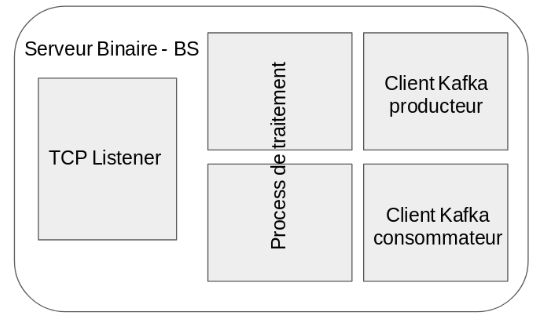
\includegraphics[scale=0.8]{\images/architecture_BS_iteration2.png}
                \caption{La conception de l'architecture du BS de l'itération 2}
                \label{Figure }
            \end{figure}
        
       
            Le BS  repose sur 3 grands composants: 
            En premier temps, le TCP serveur qui gère la connexion avec le boitier. 
            En deuxième temps,le traitement des données doit être gérer en parallèle. 
            Ce traitement assure l’encodage du protobuf boitier au protobuf cloud et 
            vis-versa. 
            D’autre part, deux clients kafka, un producteur qui va publier les messages 
            encodés et un autre consommateur qui va recevoir les messages d event. 

            \subsection{Implémentation}
            Le nouveau BS lance les diverses traitements dans des traitements en 
            parallèle. L’implémentation de ces processus parallèles s’effectuent grâce 
            aux goroutines du langage go, ce qui englobe toutes les fonctionnalités du BS 
            dans un même composant unifié.

            \subsubsection{Control plane}
             Concernant le flux de données ou Control plane, la communication entre 
             ces processus se fait comme le présente la figure \ref{Figure : controlplane}. \\

             \begin{figure}[ht]
                \centering
                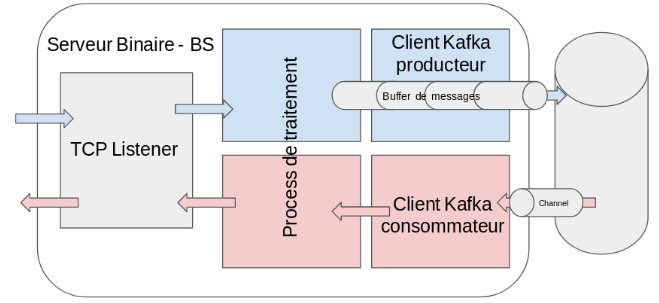
\includegraphics[scale=0.8]{\images/control_plane.png}
                \caption{Le flux de données du BS de l'itération 2}
                \label{Figure : controlplane}
            \end{figure}

            \begin{itemize}
                \renewcommand{\labelitemi}{$\bullet$}
                \item \textbf{Le boitier envoie un track pour le cloud:} \\
                La première connexion se fait avec le TCP Listener. 
                Comme son nom l’indique, ce composant écoute, vérifie et  maintient la 
                connexion avec les boîtiers. Il est considéré comme le Générateur. 
                Après avoir vérifier la connexion avec un boitier donné, il envoie le 
                message reçu au processus de traitement dans un channel. \\
                Ce dernier décode le format du message et l’encode en format des données du 
                cloud. Ensuite il le met dans un buffer des messages prêts à la publication 
                kafka. Puis le client kafka envoie tous les messages du buffer d’une manière 
                périodique de quelques secondes.\\ 
                L’envoi des messages d’une manière périodique minimise l'accès 
                écriture dans la BD ce qui augmente l’efficacité du traitement global. \\
                \item \textbf{ Le cloud envoie un event au boîtier:} \\
                Le service qui a déclenché l’event va publier dans le broker des messages le 
                message dans un topic spécifique. Le client consommateur est toujours en écoute sur ce topic, 
                il reçoit le message et l'envoie directement au traitement. Le message s’encode avec le format 
                protobuf du boitier est maintenant prêt à être envoyer au boîtier. Le TCP listener s’occupe alors 
                de son envoi à son boitier. \\
                Il est à noter que l'implémentation de cet envoi par rapport à plusieurs 
                instances sera plus complexe. 
            \end{itemize}
            


        \subsubsection{Go un language différent}
       
        Paragraphe sur le language Go : 
        Go est un jeune language de programmation système
        fascinant. Ce language compilé hérite des idées des paradigmes de
        programmation impérative et fonctionnelle. Il définit des concepts et
        des règles qui assurent à l'utilisateur des binaires .\\[0.3cm]
       
      
        Plusieurs notions de Go ont été implémenté dans le projet \gls{md30}. Parmi ces notions et Patterns :

        \begin{itemize}
            \item les Goroutines: Une fonction indépendante en cours d'exécution qui est lancé par une instruction go. 
            Cette goroutine possède sa propre call stack, qui se développe et se réduit comme requiers.
            Une goroutine est faible en cout. donc le fait de lancer des centaines voire des milliers n'est pas couteux.
            Une goroutine nest pas un thread ... Dans un programme go on peu trouver un seul thread avec plusieurs goroutines.\\

            \item la gestion Data race : \\

            \item Go conccurency pattern: Pipeline : Les primitives de concurrence de Go facilite la construction 
            des data streaming qui prouve l’efficacité d utilisation des I/O avec multiple CPUs. 
            Il n existe pas une définition formelle de pipeline. c’est une parmi plusieurs type de programme concurrentiel. D'une façon générale , une pipeline est une série d’étapes connectés par une “channel”, chaque étape est un groupe de goroutines qui exécute la même fonction. 
            Chaque étape les goroutines:

                    reçoivent une valeur de upstream depuis les channels de lectures
                    effectuent un certain traitement de fonctions sur cette valeur qui produit de nouvelle valeur 
                    envoient les nouvelles valeurs downstream pour les channels d’écriture



        \end{itemize}

    \subsection{Test }
       

    Les tests unitaires ... 
    k8s ... 

    \subsection{Amélioration à effectuer}
        Data plane et l intégration du bon protobuf.. 
        

	\section{Conclusion}

Une conclusion globale sur tous le projet, l experience ...\\
Apprendre Go était une très belle expérience. La réference principale
pour moi était .... 
... m'a servi de réference pour
comprendre des concepts sur le fonctionnement interne du language.
Mais ça m'a aidé à comprendre un certain nombre de concepts comme le parrallélisme.

\bigskip
Il faut aussi dire que le bagage fourni par les cours de compilation, d'algorithmique et de complexité à
\establishment{} était d'une utilité exceptionnelle, surtout que
programmer en Go repose sur les notions fondamentales de la programmation., \\[0.3cm]
Mais la piste principale pour l'apprentissage reste la pratique. Et avec
le projet \gls{md30} j'ai eu la chance d'approfondire des recherches,
apprendre des concepts et des patterns, et tester, dans un cycle qui a
duré 5 mois et demi. 

	\pagebreak

	% Appendix sections
	\appendix

	% Print bibliography
	\addcontentsline{toc}{section}{Bibliographie}
	\printbibliography
	\pagebreak

	% Print glossary
	\addcontentsline{toc}{section}{Glossaire}
	\glsnogroupskiptrue
	\printglossaries

\end{document}
